% Standalone TikZ figure: Actor-Critic Architecture
% For Chapter 2: Background and Theoretical Foundations
\documentclass[tikz,border=10pt]{standalone}
\usepackage{tikz}
\usetikzlibrary{arrows.meta, positioning, shapes.geometric, fit, backgrounds, calc, decorations.pathreplacing}

\begin{document}
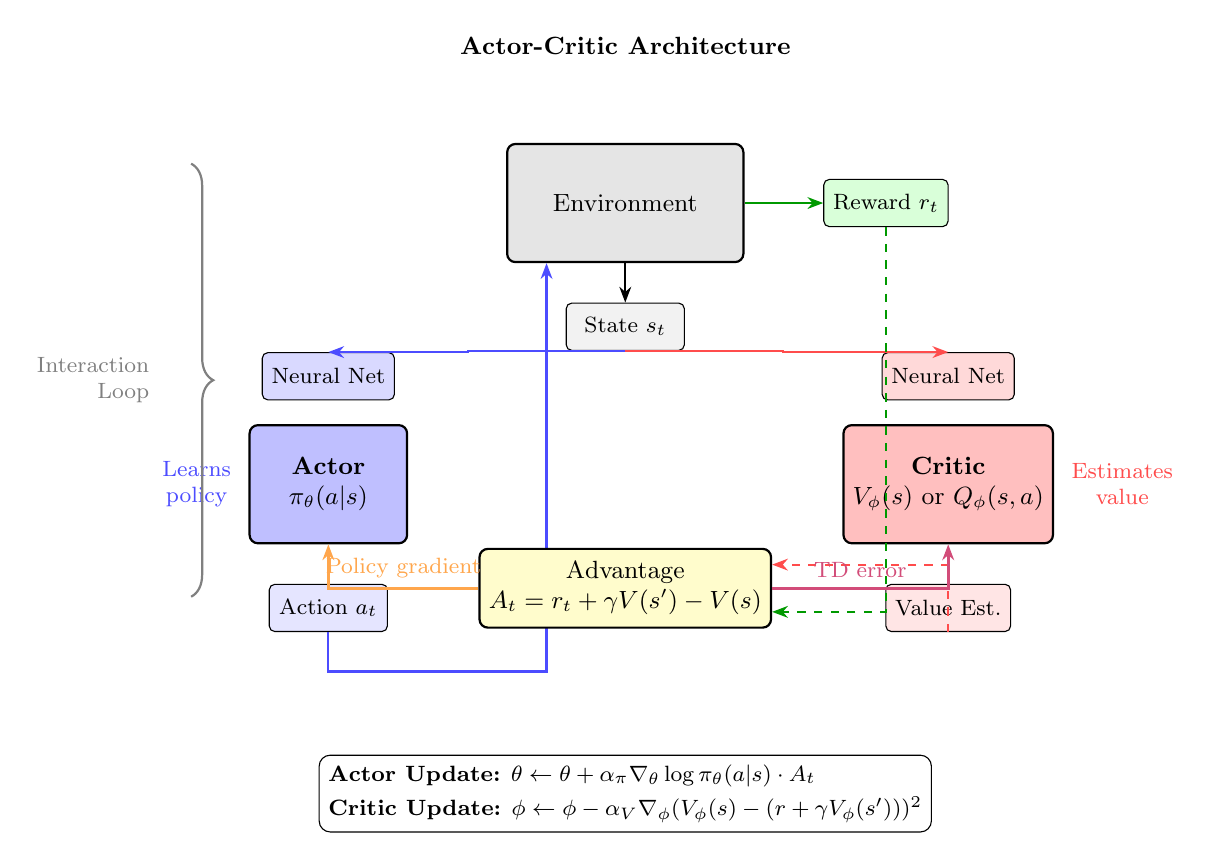
\begin{tikzpicture}[
    node distance=1cm and 1.5cm,
    every node/.style={font=\small},
    box/.style={rectangle, draw, thick, minimum width=2.2cm, minimum height=1cm, align=center, rounded corners=3pt},
    netbox/.style={rectangle, draw, thick, minimum width=2cm, minimum height=1.5cm, align=center, rounded corners=3pt},
    smallbox/.style={rectangle, draw, minimum width=1.5cm, minimum height=0.6cm, align=center, rounded corners=2pt, font=\footnotesize},
    arrow/.style={-{Stealth[length=2mm]}, thick},
    dashedarrow/.style={-{Stealth[length=2mm]}, thick, dashed},
    label/.style={font=\footnotesize},
    title/.style={font=\bfseries\small}
]

% ============ ENVIRONMENT ============
\node[box, fill=gray!20, minimum width=3cm, minimum height=1.5cm] (env) at (0, 0) {Environment};

% State output
\node[smallbox, fill=gray!10, below=0.5cm of env] (state) {State $s_t$};
\draw[arrow] (env) -- (state);

% ============ ACTOR NETWORK ============
\node[netbox, fill=blue!25, left=2cm of state, yshift=-2cm] (actor) {
    \textbf{Actor}\\
    $\pi_\theta(a|s)$
};

% Policy layers
\node[smallbox, fill=blue!15, above=0.3cm of actor] (actor_fc) {Neural Net};

% Actor output
\node[smallbox, fill=blue!10, below=0.5cm of actor] (action) {Action $a_t$};

% ============ CRITIC NETWORK ============
\node[netbox, fill=red!25, right=2cm of state, yshift=-2cm] (critic) {
    \textbf{Critic}\\
    $V_\phi(s)$ or $Q_\phi(s,a)$
};

% Critic layers
\node[smallbox, fill=red!15, above=0.3cm of critic] (critic_fc) {Neural Net};

% Critic output
\node[smallbox, fill=red!10, below=0.5cm of critic] (value) {Value Est.};

% ============ CONNECTIONS ============
% State to Actor
\draw[arrow, blue!70] (state.south) -- ++(-2, 0) |- (actor_fc.north);

% State to Critic
\draw[arrow, red!70] (state.south) -- ++(2, 0) |- (critic_fc.north);

% Actor to Environment
\draw[arrow, blue!70] (action.south) -- ++(0, -0.5) -| ([xshift=-1cm]env.south);

% Environment response
\node[smallbox, fill=green!15, right=1cm of env] (reward) {Reward $r_t$};
\draw[arrow, green!60!black] (env.east) -- (reward.west);

% ============ LEARNING SIGNALS ============
% Advantage computation
\node[box, fill=yellow!20, below=2.5cm of state, minimum width=2.5cm] (advantage) {
    Advantage\\
    $A_t = r_t + \gamma V(s') - V(s)$
};

% TD error to critic
\draw[dashedarrow, red!70] (value.south) |- ([yshift=0.3cm]advantage.east);
\draw[dashedarrow, green!60!black] (reward.south) |- ([yshift=-0.3cm]advantage.east);

% Advantage to actor update
\draw[arrow, orange!70, very thick] (advantage.west) -| node[near start, above, label] {Policy gradient} (actor.south);

% Critic update
\draw[arrow, purple!70, very thick] (advantage.east) -| node[near start, above, label] {TD error} (critic.south);

% ============ UPDATE EQUATIONS ============
\node[draw, rounded corners, fill=white, align=left, font=\footnotesize] at (0, -7.5) {
    \textbf{Actor Update:} $\theta \leftarrow \theta + \alpha_\pi \nabla_\theta \log \pi_\theta(a|s) \cdot A_t$\\[3pt]
    \textbf{Critic Update:} $\phi \leftarrow \phi - \alpha_V \nabla_\phi (V_\phi(s) - (r + \gamma V_\phi(s')))^2$
};

% ============ LABELS AND ANNOTATIONS ============
% Actor annotation
\node[label, blue!70, align=center, left=0.1cm of actor] {
    Learns\\
    policy
};

% Critic annotation
\node[label, red!70, align=center, right=0.1cm of critic] {
    Estimates\\
    value
};

% Title
\node[title] at (0, 2) {Actor-Critic Architecture};

% Feedback loop annotation
\draw[decorate, decoration={brace, amplitude=8pt}, thick, gray]
    ([xshift=-4cm, yshift=0.5cm]env.west) -- ([xshift=-4cm, yshift=-5cm]env.west)
    node[midway, left=0.4cm, align=right, font=\footnotesize] {
        Interaction\\
        Loop
    };

\end{tikzpicture}
\end{document}
